\documentclass[10pt]{scrartcl}

\usepackage[utf8]{inputenc}
\usepackage{tabularx}
\usepackage[ngerman]{babel}
\usepackage[automark]{scrpage2}
\usepackage{amsmath,amssymb,amstext}
%\usepackage{mathtools}
\usepackage[]{color}
\usepackage[]{enumerate}
\usepackage{graphicx}
\usepackage{lastpage}
\usepackage[perpage,para,symbol*]{footmisc}
\usepackage{listings} 
\usepackage[pdfborder={0 0 0},colorlinks=false]{hyperref}
\usepackage[numbers,square]{natbib}
\usepackage{color}
\usepackage{colortbl}
\usepackage{listings}
\usepackage{a4wide}
\usepackage{xspace}
\usepackage{listings}
\usepackage{hyperref}
\usepackage{epstopdf}

\lstset{numbers=left, numberstyle=\tiny, numbersep=5pt, breaklines=true, showstringspaces=false} 

%changehere
\def\titletext{TH1 Praktikum 3 : Ausarbeitung}
\def\titletextshort{Praktikum 3}
\author{Carsten Noetzel, Armin Steudte}

\title{\titletext}

%changehere Datum der Übung
\date{16.05.2012}

\pagestyle{scrheadings}
%changehere
\ihead{TH1, Padberg}
\ifoot{Generiert am:\\ \today}

\cfoot{Carsten Noetzel, Armin Steudte}


\ohead[]{\titletextshort}
\ofoot[]{{\thepage} / \pageref{LastPage}}

\setlength{\parindent}{0.0in}
\setlength{\parskip}{0.1in}

\begin{document}
\maketitle

\setcounter{tocdepth}{3}
\tableofcontents
\listoffigures
%\lstlistoflistings

\section{Aufgabe 1}
\begin{enumerate}
\item{Reversibilität / Lebendigkeit}\\
Lebendigkeit $\Rightarrow$ Reversibilität, da aus der Lebendigkeit folgt, dass es eine echt positive T-Invariante gibt für die gilt $\forall t \in T : I_{T}(t) \geq 1$. Weiterhin setzt ein lebendiges Netz voraus, dass alle $t \in T$  M-aktiviert sind, wodurch man von einer beliebigen Markierung M aus jede Transition erreichen können muss.\\
Die Umkehrung gilt nicht! Reversibilität $\nRightarrow$ Lebendigkeit

\item{Beschränktheit / Lebendigkeit}\\
Zwischen der Beschränktheit eines Netzes und seiner Lebendigkeit gibt es keinen direkten Zusammenhang. Ein Netz kann beschränkt und lebendig (Abbildung \ref{fig:BL}), beschränkt und nicht lebendig (Abbildung \ref{fig:BnL}), unbeschränkt und lebendig (Abbildung \ref{fig:nBL}) und unbeschränkt und nicht lebendig sein (Abbildung \ref{fig:nBnL}).

\begin{figure}
\begin{minipage}[hbt]{7cm}
	\centering
	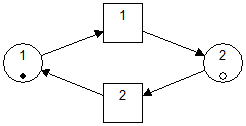
\includegraphics[width=0.7\textwidth]{Bilder/2_Beschraenkt_und_Lebendig.png}
	\caption{beschränktes und lebendiges Netz}
	\label{fig:BL}
\end{minipage}
\hfill
\begin{minipage}[hbt]{7cm}
	\centering
	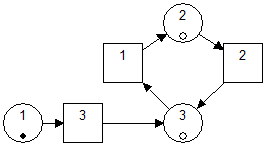
\includegraphics[width=0.7\textwidth]{Bilder/2_Beschraenkt_nicht_Lebendig.png}
	\caption{beschränktes und nicht lebendiges Netz}
	\label{fig:BnL}
\end{minipage}
\end{figure}
\begin{figure}
\begin{minipage}[hbt]{7cm}
	\centering
	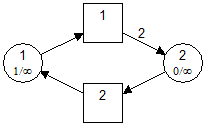
\includegraphics[width=0.7\textwidth]{Bilder/2_Nicht_Beschraenkt_und_Lebendig.png}
	\caption{nicht beschränktes und lebendiges Netz}
	\label{fig:nBL}
\end{minipage}
\hfill
\begin{minipage}[hbt]{7cm}
	\centering
	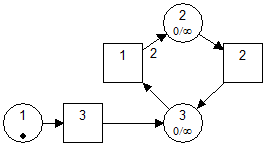
\includegraphics[width=0.7\textwidth]{Bilder/2_Nicht_Beschraenkt_nicht_Lebendig.png}
	\caption{nicht beschränktes und nicht lebendiges Netz}
	\label{fig:nBnL}
\end{minipage}
\end{figure}

\item{Beschränktheit / Reversibilität}\\
Reversibilität $\Rightarrow$ Beschränktheit, da der Erreichbarkeitsgraph des Netzes endlich sein muss, weil $\forall M \in EG$ gilt: $M_{0} \overset{*}{\rightarrow} M \overset{*}{\rightarrow} M_{0}$. Das heißt, das Netz muss aus jeder beliebigen Markierung wieder zurück zur Anfangsmarkierung kommen, was bei unbeschränkten Netzen nicht möglich ist.\\
Die Umkehrung gilt nicht! Beschränktheit $\nRightarrow$ Reversibilität

\item{Erreichbarkeit / Lebendigkeit}\\
Lebendigkeit $\Rightarrow$ Erreichbarkeit\\
Wenn ein $t \in T$ lebendig ist, muss es $\forall M \in EG$ M-erreichbar sein, daraus folgt $\exists M \in EG$ für das gilt t ist aus M erreichbar.\\
Wenn das Netz lebendig ist, sind alle Transitionen lebendig und damit $\forall M \in EG$ M-erreichbar.

\item{Erreichbarkeit / Reversibilität}\\

\item{Erreichbarkeit / Beschränktheit}\\

\item{Stelleninvarianten / Lebendigkeit}\\

\item{Stelleninvarianten / Reversibilität}\\

\item{Stelleninvarianten / Beschränktheit}\\

\item{Stelleninvarianten / Erreichbarkeit}\\

\item{Transitionsinvarianten / Lebendigkeit}\\

\item{Transitionsinvarianten / Reversibilität}\\

\item{Transitionsinvarianten / Beschränktheit}\\

\item{Transitionsinvarianten / Erreichbarkeit}\\

\item{Transitionsinvarianten / Stelleninvarianten}\\

\item{Überdeckungsgraph / Lebendigkeit}\\

\item{Überdeckungsgraph / Reversibilität}\\

\item{Überdeckungsgraph / Beschränktheit}\\

\item{Überdeckungsgraph / Erreichbarkeit}\\

\item{Überdeckungsgraph / Stelleninvarianten}\\

\item{Überdeckungsgraph / Transitionsinvarianten}\\

\item{Kondensation des EG / Lebendigkeit}\\

\item{Kondensation des EG  / Reversibilität}\\

\item{Kondensation des EG  / Beschränktheit}\\

\item{Kondensation des EG  / Erreichbarkeit}\\

\item{Kondensation des EG  / Stelleninvarianten}\\

\item{Kondensation des EG  / Transitionsinvarianten}\\

\item{Kondensation des EG  / Überdeckungsgraph}\\

\item{Verklemmung / Lebendigkeit}\\

\item{Verklemmung / Reversibilität}\\

\item{Verklemmung / Beschränktheit}\\

\item{Verklemmung / Erreichbarkeit}\\

\item{Verklemmung / Stelleninvarianten}\\

\item{Verklemmung / Transitionsinvarianten}\\

\item{Verklemmung / Überdeckungsgraph}\\

\item{Verklemmung / Kondensation des EG}\\

\end{enumerate}
\textbf{Reversibilität / Lebendigkeit}


\section{Aufgabe 2}

\end{document}

